\section{High Band Improvement}
From the S-parameter measurements of both the triangle feed antenna and the minimized monopole antenna, it is clear that both antennas are experiencing problems in the high band when moved from simulation to the PCB with tuner.

It has been chosen to elaborate on the minimized monopole antenna design and improve the high band. In order to do so, a second set of arms has been added to the antennas as shown in Figure~\ref{fig:sparam_5mm_highband}. As previous experience has shown that the simplified simulations will detune in practice, the matching components in Figure~\ref{fig:sparam_5mm_highband} have been chosen to resonate slightly higher than desired. 

\begin{figure}[htbp]
    \begin{subfigure}[b]{0.49\linewidth}
        \centering
        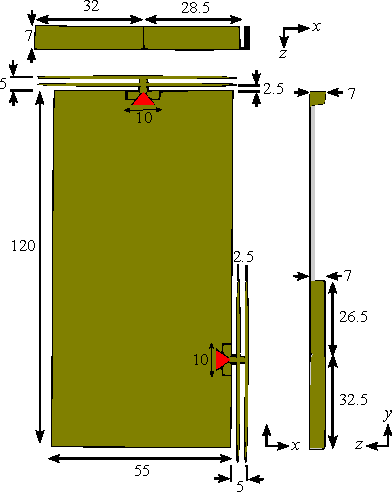
\includegraphics{img/tech_sol/monopole/highband/3d_drawing}
        \caption{Technical drawing.}
        \label{fig:ant1technical_highband}
    \end{subfigure}
    \hfill
    \begin{subfigure}[b]{0.49\linewidth}
        \centering
        \includegraphics{img/tech_sol/schematic_tuning_1}\\[1cm]
\footnotesize
        \begin{tabular}{|l|l|l|l|}
            \hline
            & $C_1$ & $L_1$ & $C_2$ \\
            \hline
            Top antenna & \SI{3.02}{pF} & \SI{7.99}{nH} & $[0.3,2.9]\,$pF\\
            Side antenna & \SI{1.81}{pF} & \SI{5.27}{nH} & $[0.3,2.9]\,$pF\\
            \hline
        \end{tabular}
        \caption{Tuning/matching circuit.}
        \label{fig:ant1_tuning_highband}
    \end{subfigure}
    \caption{Technical drawing and tuning circuit for the antenna.  The matching circuit is applied for both the top and the side antenna.}
    \label{fig:sparam_5mm_highband}
\end{figure}

\FloatBarrier
\subsection{Simulation}

The new antenna design presented in Figure~\ref{fig:sparam_5mm_highband} has been simulated. The resulting S-parameter sweep can be seen in Figure~\ref{fig:sparam_mono_modi_sim}. The low band of both antennas can be covered by sweeping the tuning capacitor. The high band resonates higher than desired but is likely to detune when the antennas are added to the PCB.

% Sweeping S-parameters
\begin{figure}[htbp]
   \begin{subfigure}[b]{0.49\linewidth}
        \centering
        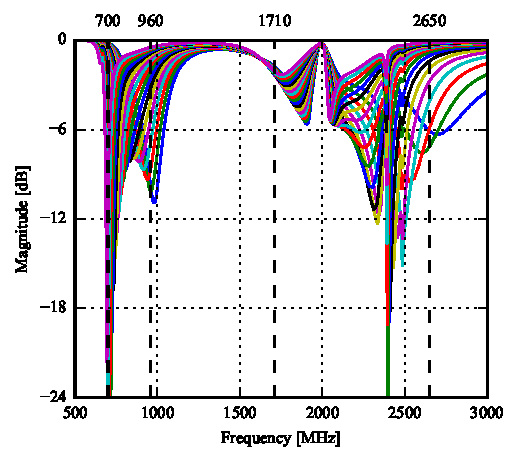
\includegraphics{img/tech_sol/monopole/highband/sim/s11.pdf}
        \caption{$S_{11}$, sweeping $C_1$ and fixing $C_2$.}
   \end{subfigure}
    \hfill
    \begin{subfigure}[b]{0.49\linewidth}
        \centering
        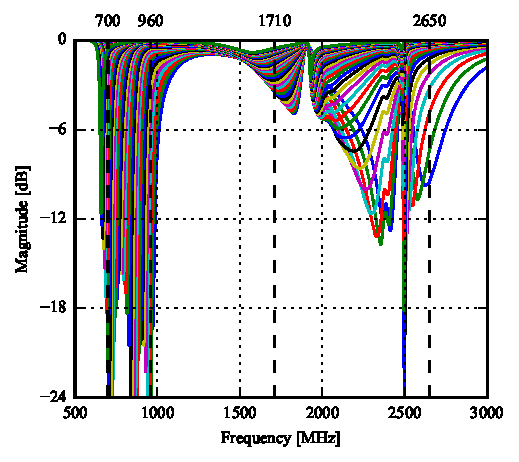
\includegraphics{img/tech_sol/monopole/highband/sim/s22.pdf}
        \caption{$S_{22}$, sweeping $C_2$ and fixing $C_1$.}
    \end{subfigure}
~
    \begin{subfigure}[b]{0.49\linewidth}
        \centering
        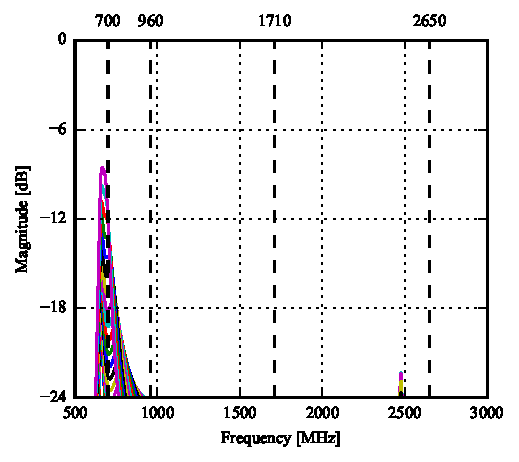
\includegraphics{img/tech_sol/monopole/highband/sim/s11_s21.pdf}
        \caption{$S_{21}$, sweeping $C_1$ and fixing $C_2$.}
    \end{subfigure}
    \hfill
    \begin{subfigure}[b]{0.49\linewidth}
        \centering
        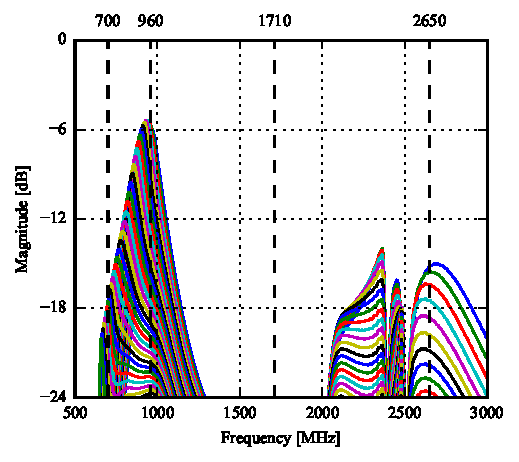
\includegraphics{img/tech_sol/monopole/highband/sim/s22_s21.pdf}
        \caption{$S_{21}$, sweeping $C_2$ and fixing $C_1$.}
    \end{subfigure}
    \caption{S-parameter sweep in free space for tuning the shunt capacitor of each antenna, $C_1$ and $C_2$ for port 1 and 2, respectively. Port 1 is the top antenna and port 2 is the side antenna.}
    \label{fig:sparam_mono_modi_sim}
\end{figure}

\FloatBarrier
\subsection{User Effect Simulations}

\FloatBarrier
\subsection{Measurements}

\begin{figure}[htbp]
        \centering
        \begin{tabular}{m{3in}m{3in}}
            \centering
            \includegraphics{img/tech_sol/schematic_tuning_1}&
            \centering
            \footnotesize
            \begin{tabular}{|l|l|l|l|}
                \hline
                & $C_1$ & $L_1$ & $C_2$ \\
                \hline
              Top antenna & \SI{3.9}{pF} & \SI{2.2}{nH} & \SI{0.6}{pF} \\
              Side antenna & \SI{4}{pF} & \SI{1}{nH} & \SI{1.2}{pF} \\
                \hline
            \end{tabular}
        \end{tabular}
    \caption{Matching circuit for the minimized monopole prototype. These are the component values where the bandwidth is found to be the largest.}
    \label{fig:mono_matching_modi_meas}
\end{figure}

\begin{figure}[htbp]
    \centering
    \begin{subfigure}{0.49\linewidth}
        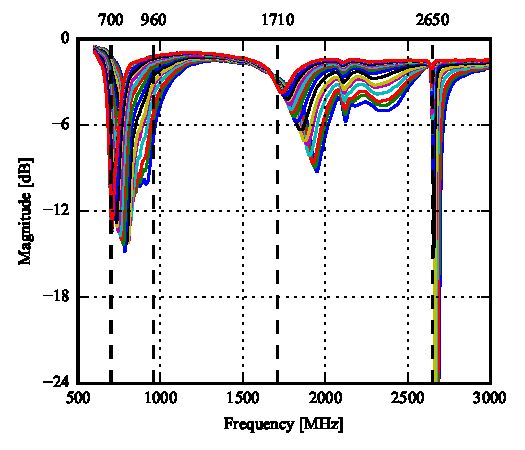
\includegraphics{img/tech_sol/monopole/highband/meas/tuner/S11.pdf}
        \caption{S11.}
    \end{subfigure}
    \hfill
    \begin{subfigure}{0.49\linewidth}
        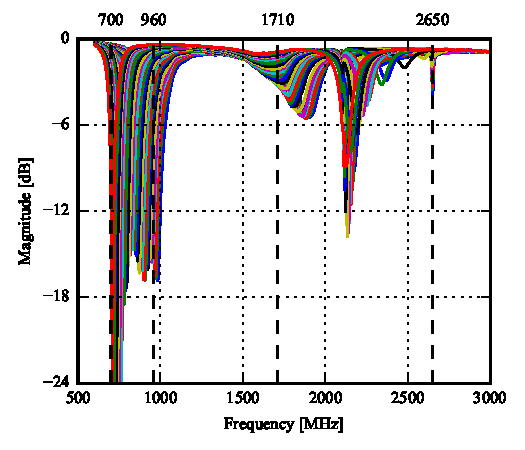
\includegraphics{img/tech_sol/monopole/highband/meas/tuner/S22.pdf}
        \caption{S22.}
    \end{subfigure}
    \\
    \begin{subfigure}{0.49\linewidth}
        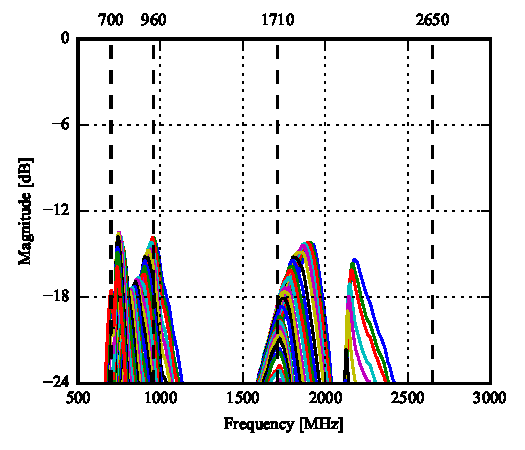
\includegraphics{img/tech_sol/monopole/highband/meas/tuner/S21.pdf}
        \caption{S21.}
    \end{subfigure}
    \caption{S-parameters for the modified minimized monopole prototype. The top-tuner is swept from approximately \SI{0.6}{pF} to \SI{6}{pF} and the side-tuner is swept from approximately \SI{1.2}{pF} to \SI{12}{pF}. The two tuners are tracking the first half of the sweep.}
    \label{fig:sparam_mono_modi_meas}
\end{figure}

\FloatBarrier
\subsection{Final Design and Measurements}
In this section, the final design with all above mentioned improvements will be presented. The design is shown in Figure~\ref{fig:final_lassedouble}, and dimensions of the antenna elements are the same as shown in Figure~\ref{fig:sparam_5mm_highband}. As shown in Figure~\ref{fig:final_lassedouble}, a capacitor has been added on each transmission line (from SMA to matching network), improving the return loss significantly. The matching network is nearly the same as in Figure~\ref{fig:mono_matching_modi_meas}. The exact component values are printed on Figure~\ref{fig:final_lassedouble}.

\begin{figure}[htbp]
    \centering
    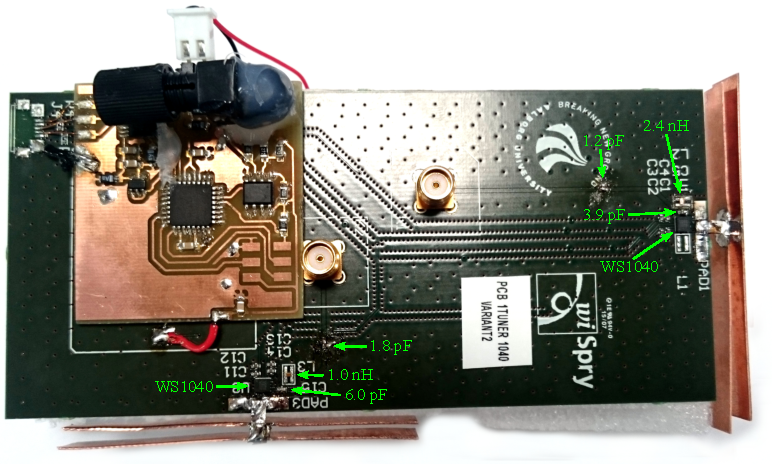
\includegraphics{img/tech_sol/monopole/highband/meas/final_tuner/lassedouble.pdf}
    \caption{Final antenna design with capacitors added to the transmission line to improve high-band performance.}
    \label{fig:final_lassedouble}
\end{figure}

\begin{figure}[htbp]
    \centering
    \begin{subfigure}{0.49\linewidth}
        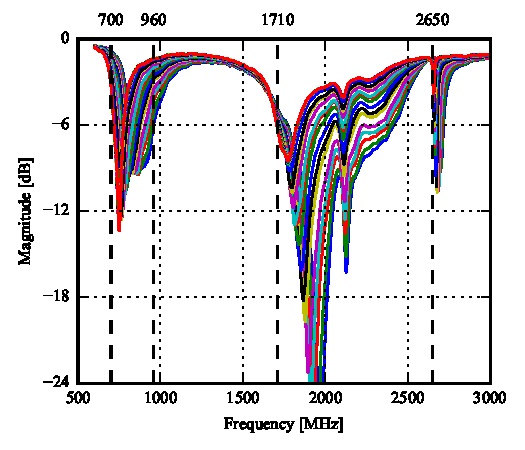
\includegraphics{img/tech_sol/monopole/highband/meas/final_tuner/S11.pdf}
        \caption{S11.}
    \end{subfigure}
    \hfill
    \begin{subfigure}{0.49\linewidth}
        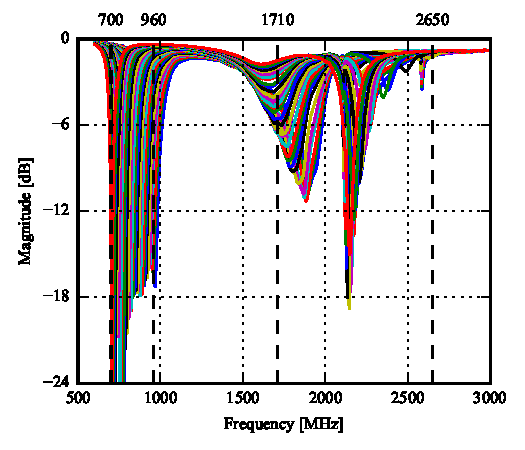
\includegraphics{img/tech_sol/monopole/highband/meas/final_tuner/S22.pdf}
        \caption{S22.}
    \end{subfigure}
    \\
    \begin{subfigure}{0.49\linewidth}
        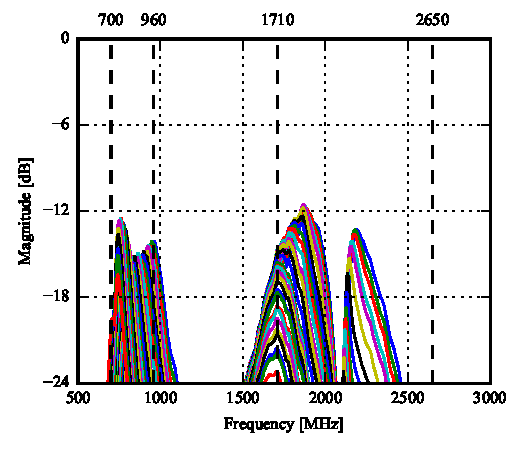
\includegraphics{img/tech_sol/monopole/highband/meas/final_tuner/S21.pdf}
        \caption{S21.}
    \end{subfigure}
    \caption{S-parameters of the final antenna design. The top antenna is swept from approximately \SI{0.6}{pF} to \SI{6}{pF} and the side antenna from approximately \SI{1.2}{pF} to \SI{12}{pF}. The tuners are tracking the first half of the sweep.} 
    \label{fig:final_sparams}
\end{figure}

\begin{figure}[htbp]
    \centering
    \begin{subfigure}{0.49\linewidth}
        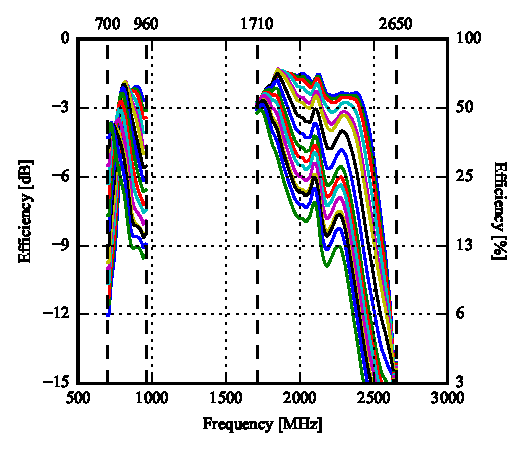
\includegraphics{img/tech_sol/monopole/highband/meas/final_tuner/efficiency_top.pdf}
        \caption{Top antenna.}
    \end{subfigure}
    \hfill
    \begin{subfigure}{0.49\linewidth}
        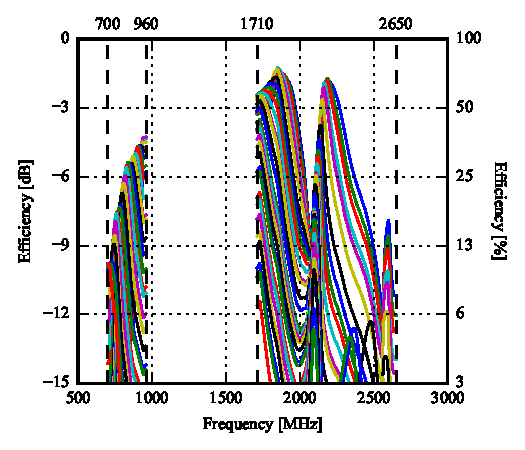
\includegraphics{img/tech_sol/monopole/highband/meas/final_tuner/efficiency_side.pdf}
        \caption{Side antenna.}
    \end{subfigure}
    \caption{Total efficiency of the final antenna design. The top antenna is swept from approximately \SI{0.6}{pF} to \SI{6}{pF} and the side antenna from approximately \SI{1.2}{pF} to \SI{12}{pF}. The tuners are tracking the first half of the sweep.}
    \label{fig:final_efficiency}
\end{figure}

%%%%%%%%%%%%%%%%%%%%%%%%%%%%%%%%%%%%%%%%%%%%%%%%%%%%%%%%%%%%%%%%%%%%%%%%%%%%%%%%
% Henrik og Lasse: I skal under ingen omstændigheder kopiere teksten nedenfor.
% Der går noget galt hvis I prøver! Skriv noget fra bunden i stedet!
%%%%%%%%%%%%%%%%%%%%%%%%%%%%%%%%%%%%%%%%%%%%%%%%%%%%%%%%%%%%%%%%%%%%%%%%%%%%%%%%

The measured S-parameters are shown in Figure~\ref{fig:final_sparams}. For the top antenna, the tunable bandwidth in the low band (by \SI{960}{MHz}) is \SI{140}{MHz} and can be swept all the way down to \SI{700}{MHz}. The high band can be covered from \SI{1710}{MHz} to around \SI{2450}{MHz}. There is still a problem covering the band from \SI{2550}{MHz} to \SI{2650}{MHz} but all bands from \SI{700}{MHz} to \SI{2400}{MHz} can be covered. For the side antenna, the tunable bandwidth by \SI{960}{MHz} is \SI{70}{MHz} and can be swept all the way down to \SI{700}{MHz}. The high band covers from \SI{1710}{MHz} to \SI{1975}{MHz} and from \SI{2095}{MHz} to \SI{2275}{MHz}.

The measured efficiency is shown in Figure~\ref{fig:final_efficiency}. The top antenna is able to cover the low band at \SI{-4}{dB} efficiency and the high band at \SI{-3}{dB} from \SI{1710}{MHz} to \SI{2430}{MHz}. The side antenna is not as good and is only able to cover the low band at and efficiency between \SI{-10}{dB} to \SI{-4}{dB}. The high band has two resonances and is covered at \SI{-3}{dB} from \SI{1710}{MHz} to \SI{1960}{MHz} and from \SI{2130}{MHz} to \SI{2260}{MHz}. Both shown a problem covering the very highest bands above \SI{2550}{MHz}.

%%%%%%%%%%%%%%%%%%%%%%%%%%%%%%%%%%%%%%%%%%%%%%%%%%%%%%%%%%%%%%%%%%%%%%%%%%%%%%%%
%%%%%%%%%%%%%%%%%%%%%%%%%%%%%%%%%%%%%%%%%%%%%%%%%%%%%%%%%%%%%%%%%%%%%%%%%%%%%%%%


